\documentclass{beamer}

\setlength{\parskip}{\baselineskip}
\setlength{\parindent}{0pt}
\usepackage{default}
\usepackage{tabularx}
\usepackage{url}
\usepackage{graphicx}
\usepackage{listings}
\usepackage{color}
\usepackage{amssymb,amsmath,amsthm,mathrsfs,mathtools,amscd}
\usepackage{mathrsfs}

\definecolor{darkgreen}{rgb}{0,0.6,0}

\newenvironment{recap}{\begin{small}\color{gray}\begin{flushright}}{\end{flushright}\end{small}}


\title{\huge{Citation Management with \texttt{JabRef}}}
\author{\textbf{Manuel Baumann}, Jan Heiland}
\titlegraphic{
   
\includegraphics[scale=0.08]{images/TU_Delft_logo1.png}\hspace{4cm}
\includegraphics[scale=0.15]{../../images/logo}}
\date{\footnotesize{December 19, 2013}}

\begin{document}

\frame{\titlepage}

\begin{frame}[fragile]
\frametitle{\LaTeX \ and bib-files}
How bibtex is used in \LaTeX:
\vspace{1cm}
\begin{small}
\lstset{language=[LaTeX]TeX,
texcsstyle=*\bf\color{blue},
numbers=none,
breaklines=true,
keywordstyle=\color{darkgreen},
commentstyle=\color{darkgreen},
frame=none,
tabsize=2}
\begin{lstlisting}
\documentclass{article}
\usepackage{hyperref}	    % very fancy; else:'cite'

\begin{document}

blabla, cf. \cite{GSZ11}  % cite a reference

\bibliography{my_bib}     % use file 'my_bib.bib'
\bibliographystyle{plain}

\end{document}
\end{lstlisting}
\end{small}
\end{frame}

\begin{frame}
\frametitle{What is Project baNaNa ?}
\framesubtitle{More details...}
In more detail, we were thinking about
\begin{itemize}
 \item possible topics:
 \begin{itemize}
 \item Python
 \item CUDA/OpenCL
 \item Open Foam
 \item MPI/OpenMP
 \item latex `best practice'
 \item high end Matlab usage
 \end{itemize}
 \item a classical lecture:
  \begin{itemize}
 \item approx. 20 mins
 \item once a month
 \item everybody contributes from time to time
 \item \textbf{gives many examples}
 \end{itemize}
\end{itemize}
\end{frame}

\begin{frame}
\frametitle{Today's lecture: \texttt{git}}
Do you know this situation?
\begin{figure}
\centering
 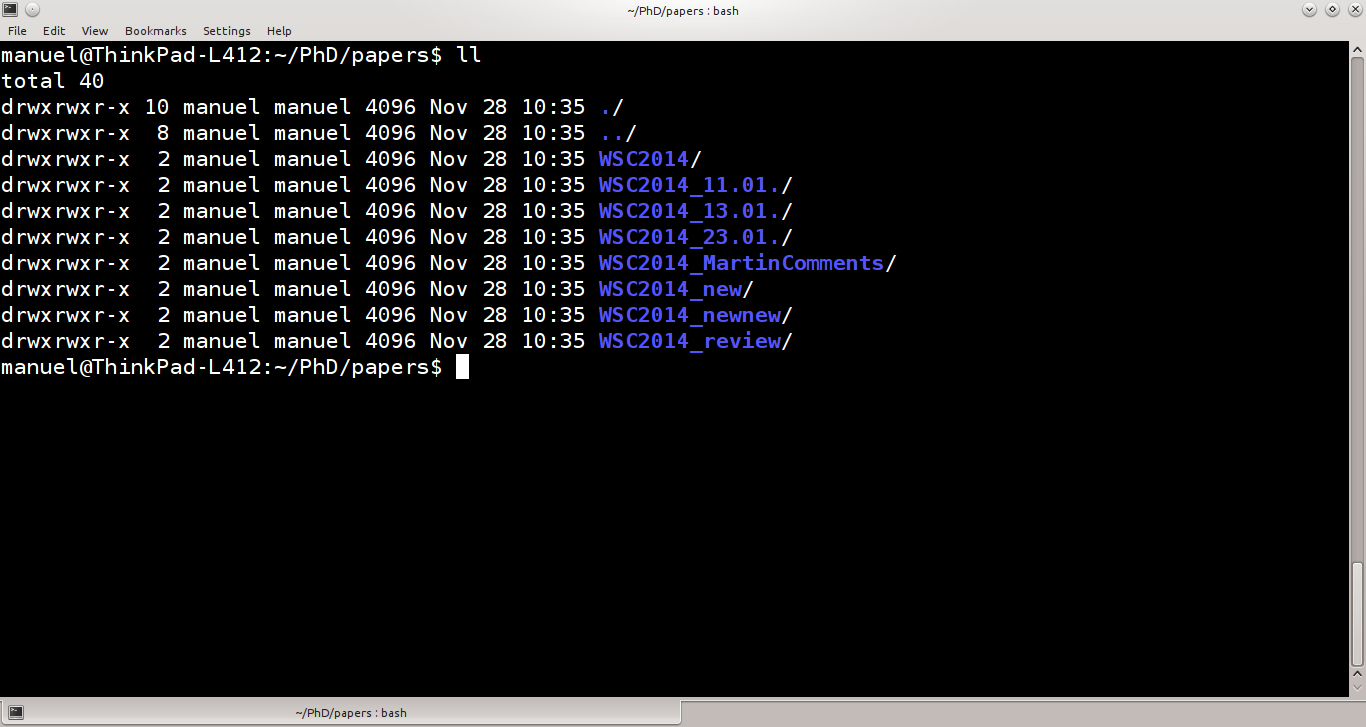
\includegraphics[height=0.6\textheight]{images/screnshot1.png}
\end{figure}
\end{frame}

\begin{frame}
\frametitle{Today's lecture: \texttt{git}}
The pre-installed software package \texttt{git} can be used for version control for a (bigger) software project.
\begin{itemize}
 \item helps to keep track of changes in your project directory
 \item branching, merging
 \item collaboration
 \item several sites allow you to publish your \texttt{git} repository (github, bitbucket, gitorious) 
\end{itemize}
\end{frame}

\begin{frame}
\frametitle{Git basics}
Git stores snapshots (called \emph{commits} in git) of files in a repository.

A commit consists of
\begin{itemize}
 \item a set of files,
 \item a message,
 \item an author,
 \item a date,
 \item references to one or more parent commits and
 \item a hash (of the above).
\end{itemize}

You are in control of creating commits!
\end{frame}

\begin{frame}[fragile]
\frametitle{Git basics}
\begin{description}[working directory]
 \item[working directory]
  Plain directory where you can edit files using your favourite editor.
 \item[staging area]
  Area listing the files to be commited.
 \item[repository]
  Collection of commits.
\end{description}

Everything is stored locally (in the working directory):
\begin{description}[working directory]
 \item[repository] \verb|working_directory/.git|
 \item[staging area] \verb|working_directory/.git/index|
\end{description}
\end{frame}

\begin{frame}
\frametitle{Basic commands}
\begin{table}
\begin{tabularx}{\textwidth}{l|X}
Command & Meaning \\
 \hline
 \texttt{git init} & First command, makes current folder a \texttt{git} repository\\
 \texttt{git add <file>} & Stages a file\\
 \texttt{git commit -m <message>} & Record changes to the repository\\
 \texttt{git status} & Show the working tree status\\
 \texttt{git diff} & Show changes between commits, commit and working tree, etc\\
 \texttt{git log} & Show commit logs\\
\end{tabularx}
\end{table}
\hfill $\hookrightarrow$ live demonstration...
\end{frame}

\begin{frame}
\frametitle{Branches}
\begin{itemize}
 \item Branching is the git-equivalent of making a copy of your working
 directory.
 \item Branching is cheap.  Use it whenever you can.
 \item Git is very good in merging (two or more) branches.
 \item NOTE: Your working directory points to only one branch.
\end{itemize}
\end{frame}

\begin{frame}
\frametitle{Commands for branching and merging}
\begin{table}
\begin{tabularx}{\textwidth}{l|X}
Command & Meaning \\
 \hline
 \texttt{git branch} & List, create, or delete branches\\
 \texttt{git checkout} & Checkout a branch or paths to the working tree\\
 \texttt{git merge} & Join two or more development histories together\\
 \texttt{git mergetool} & Run merge conflict resolution tools to resolve merge conflicts\\
\end{tabularx}
\end{table}
\hfill $\hookrightarrow$ live demonstration...
\end{frame}
\begin{frame}
\frametitle{Today's message}

The overall message is:
\begin{center}
 \textit{Using git is optimal for collaborations and big software projects.}
\end{center}
Moreover,
\begin{itemize}
 \item sensitive information should not be stored in e.g. Dropbox
 \item \texttt{git} branches are non-linear in time
 \item local argument: \texttt{git} is supported (and pre-installed) at TU Delft work stations
\end{itemize}
\end{frame}
\begin{frame}
\frametitle{Further reading}
Many information are available online:
\begin{itemize}
 \item \url{https://github.com/}
 \item \url{http://try.github.io/levels/1/challenges/1}
 \item \url{http://git-scm.com/book}
\end{itemize}
These slides, and much more, will be published at:
\begin{itemize}
 \item \url{http://projectbanana.github.io/}
\end{itemize}
 \begin{figure}
\centering
 
\includegraphics[height=0.3\textheight]{../../images/logo}
\end{figure}
\end{frame}

\end{document}
